\documentclass[18pt, a3paper, portrait]{tikzposter}
\usepackage[utf8]{inputenc}
\usepackage{blindtext}
\usepackage{comment}
\usepackage{amsmath,amsfonts,amsthm,bm} % Math packages 
\usepackage{tikz} % To make cool diagrams
\usepackage{booktabs} % For fancy tables

\newcommand{\ra}[1]{\renewcommand{\arraystretch}{#1}} % Something about allowing more space between rows in fancy tables.

\makeatletter
\def\title#1{\gdef\@title{\scalebox{\TP@titletextscale}{%
\begin{minipage}[t]{\linewidth}
\centering
#1
\par
\vspace{0.5em}
\end{minipage}%
}}}
\makeatother

\title{Whole-series Time-series Clustering Techniques}
\author{Yohann Jacob Sandvik}
\date{\today}
\institute{Institute of Electronic Systems - NTNU}
 
\usetheme{Envelope}
 
\begin{document}
 
\maketitle 
%% Overview of whole-series time-series clustering techniques
\begin{columns}
    \column{0.7}
    \block{Overview of Whole-series Time-series Clustering Techniques}
    {
        \begin{itemize}
            \item There are three types of time-series clustering, \textit{whole-series time-series clustering}, \textit{subsequence time-series clustering} and \textit{time-point time-series clustering}.
            \item In this review we will only consider work using whole-series time-series clustering.
            \item Whole series time-series clustering can broadly be divided into three main approaches. The raw-data based approach, the feature-based approach and the model based approach.
            \item When clustering raw time series the majority of the work goes into selection of similarity metric and clustering algorithm, and one clusters the time series with regard to similarity in time or similarity in shape.
            \item In the feature-based approach one also clusters time series with regard to similarity in time, and shape, but the work is somewhat shifted away from choice of similarity metric and over to choice of representation.
            \item In the model-based approach the goal is most often to cluster time series with regard to the underlying data generating process. The underlying assumption being that two time series that appear different might still have been generated by the same process.
        \end{itemize}
    }
 
    \column{0.3}
    \block{~}
    {
        \begin{tikzfigure}
            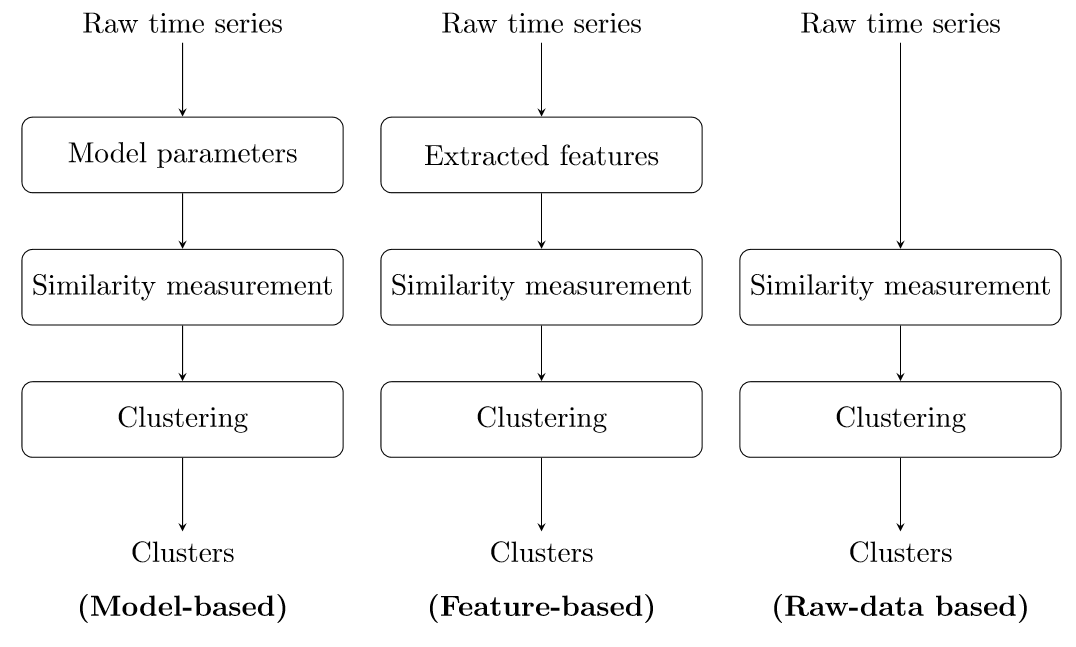
\includegraphics[width=0.25\textwidth]{images/tsc_appraches.png}
        \end{tikzfigure}
    }
\end{columns}

%% Explanation of the most common models
\begin{columns}
    \column{0.33}
    \block{ARMA models}
    {
        \begin{equation}
            X_t - \phi_1 X_{t-1} - ... - \phi_p X_{t-p} = Z_{t} + \theta_1 Z_{t-1} + ... + \theta_q Z_{t-q}
        \end{equation}
    }

    \column{0.33}
    \block{Hidden Markov Models}
    {
        Transition probabilities.
        \begin{equation}
            \begin{split}
                p_{ij}  &= P(X_n = i | X_{n-1} = i_{n-1},..., X_{0} = i_{0}) \\
                        &= P(X_n = i | X_{n-1} = i_{n-1})      
            \end{split}
            \label{eq:markov_property}
        \end{equation}
        Hidden states with emmission probabilities.
        \begin{equation}
            P(S = s | X = j)
        \end{equation}
    }

    \column{0.33}
    \block{PCA and ICA}
    {
        PCA and ICA are both ways of projecting the input matrix onto a reduced feature space.
        In PCA one finds the principal components that are the eigenvectors of the covariance matrix if the input vectors.
        In ICA one assumes that the matrix of observed variables is a linear combination of mutually independent variables.
        Hence, one tries to reconstruct a set of variables that are as ''mutually independent'' as possible.

    }
\end{columns}

%% Representation results
\begin{columns}
    \column{0.5}
    \block{Feature-based representations}
    {
        \begin{tikzfigure}
            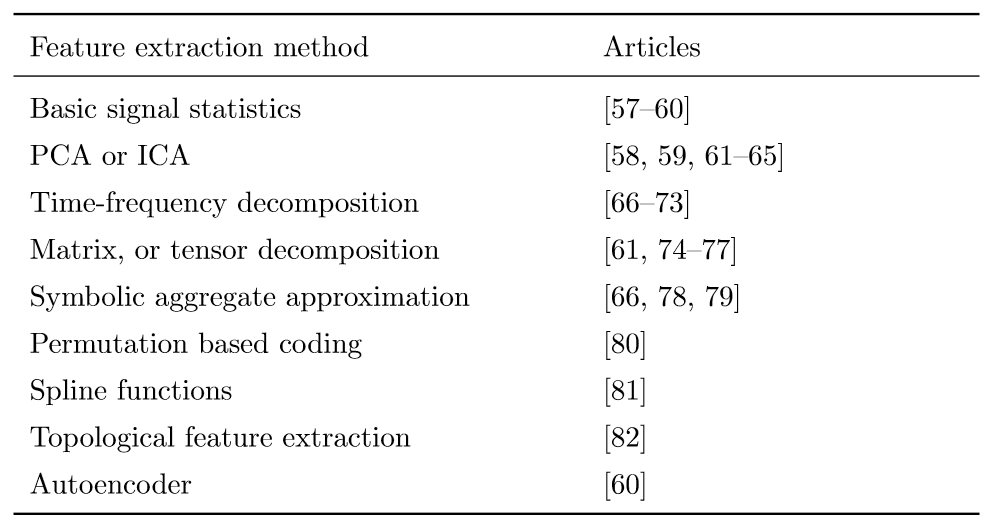
\includegraphics[width=0.4\textwidth]{images/feature_based_rep_meth_table.png}
        \end{tikzfigure}
    }
    \begin{subcolumns}
    \subcolumn{0.5}
    \block{K-means}
    {
        \begin{itemize}
            \item Family of hard clustering algorithms.
            \item Number of clusters -> predetermined.
            \item Iterative algorithm. 
            \item Not deterministic.
        \end{itemize}
    }

    \subcolumn{0.5}
    \block{Fuzzy C-means}
    {
        \begin{itemize}
            \item Family of soft clustering algorithms.
            \item Number of clusters -> predetermined.
            \item Iterative algorithm. 
            \item Not deterministic.
        \end{itemize}
    }
    \end{subcolumns}
 
    \block{Discussion}
    {
        \begin{itemize}
            \item PCA and ICA are considered to be the most viable options for feature-based representations. Because they
                build on strong theoretical ground, without being overly complex methods they are fairly interpretable.
            \item Of the model-based representation methods ARMA models were found to be a frequent model
                used. Since they are also frequently used for feature extraction in wind turbine monitoring they should be considered for a master thesis.
            \item The HMM is a model-based approach that has showed great promise in terms of
                representing time series, and has even be used to cluster the time series [91] in a simple manner.
            \item SOMs have been shown to work well on financial time series by [57, 93], so they
                could be appropriate for the time series produced by wind turbines. However, ANNs in general
                require careful design and and long training, so it might take a lot of time away that could be
                used for testing other approaches. So SOM should not be considered as a primary model-based
                clustering approach for wind turbine time series.
        \end{itemize}
    }

    \column{0.5}
    \block{Model-based representations}
    {
        \begin{tikzfigure}
            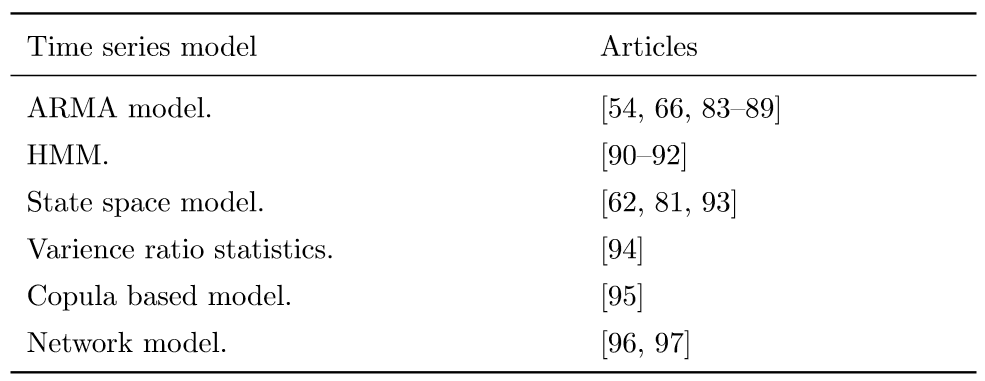
\includegraphics[width=0.4\textwidth]{images/model_based_rep_meth_table.png}
        \end{tikzfigure}
        % \vspace{3cm}
    }
    \begin{subcolumns}
    \subcolumn{0.5}
    \block{Hierarchical Clustering}
    {
        \begin{itemize}
            \item Family of hard clustering algorithms.
            \item Number of cluster -|> predetermined.
            \item Builds hierarchies of clusters.
            \item Similarity between clusters is defined by distance metric, and \textit{linkage}.
            \item Deterministic.
        \end{itemize}
    }

    \subcolumn{0.5}
    \block{Expectation Maximization}
    {
        \begin{itemize}
            \item Iterative algorithm used for estimating model parameters satisfying the ML criterion.
            \item Is used for clustering by letting each cluster being a generative process.
            \item Time and storage complexity increase exponentially with time-series length.
        \end{itemize}
    }
    \end{subcolumns}
    \block{Clustering Algorithms}
    {
        \begin{tikzfigure}
            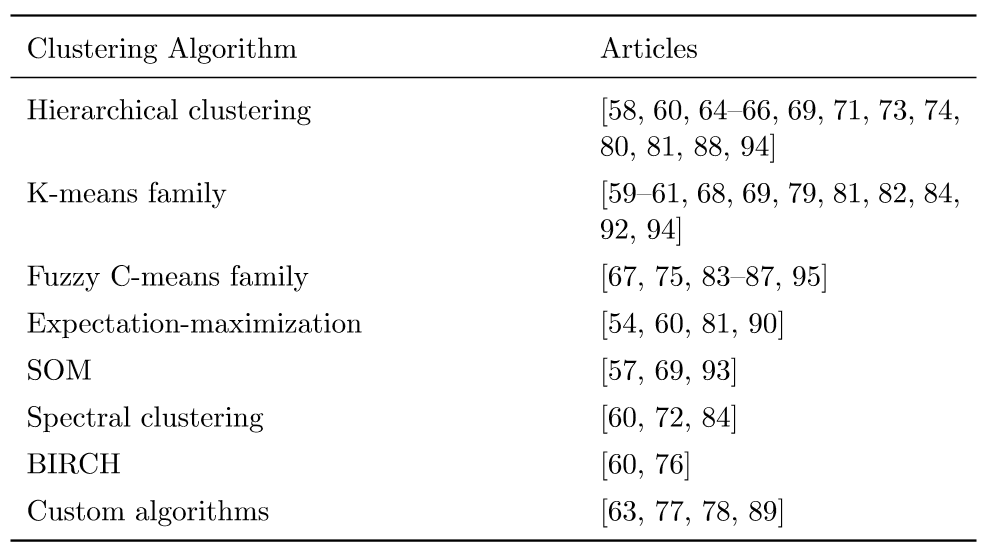
\includegraphics[width=0.45\textwidth]{images/clustering_algorithms_table.png}
        \end{tikzfigure}
    }
\end{columns}

\end{document}


